\chapter{System Requirements} \label{ch:SystemRequirements}
The user segment that this project is interested in, is the hobbyist segment. The hobbyist segment is anyone with an interest in developing electronic circuits, whether or not they have a technical or engineering background. The hobbyist segment is interested in more capable impedance analyzers than what is available in their price range as seen in section \ref{sec:ProfessionalMarketDemand}. This section has compiled a list of system requirements for an impedance analyzer that will be developed in this project. The requirements are based on the market demands in section \ref{sec:ProfessionalMarketDemand} and the currently available functions in high-end impedance analyzers shown in section \ref{sec:CommercialImpedanceMeasurement}, specifically the R\&S LCX-200, and the personal requirements from the authors of this report. 

The specific requirements can be seen in table \refq{tab:5_SystemRequirements}. 
\begin{table}[H]
    \begin{tabular}{|m{3.5em}|m{15em}|m{15em}|}
    \hline
      \textbf{ID} &   \textbf{Description}       & \textbf{Requirement}  \\ \hline
      §1 & Frequency range &    \SIQ{50}{\hertz} - \SIQ{1}{\mega\hertz}, \SIQ{1}{\hertz} resolution \\ \hline
      §2 & Impedance fit$^1$ & Series and parallel mode \\\hline 
      §3 & Impedance range & $\SIQ{10}{\milli\ohm}\leq|Z|\leq\SIQ{100}{\mega\ohm}$ \\ \hline
      §4 & $|Z|$, Modulus accuracy$^2$& $A_Z(f_m, Z_m)$ \\ \hline
      §5 & $\angle\phi$, Accuracy of argument$^3$ & $A_\phi(f_m, Z_m)$ \\ \hline
      §6 & Test voltage range & \SIQ{10}{\milli\volt}$_{pp}$ - \SIQ{5}{\volt}$_{pp}$, \SIQ{10}{\milli\volt} resolution \\ \hline
      §7 & Maximum test current & \SIQ{100}{\milli\ampere}$_{pp}$ \\ \hline
      §8 & DC bias voltage range & \SIQ{0}{\volt}DC - \SIQ{20}{\volt}DC \\ \hline
      §9 & Parameters of DUT & $L/C/R/Q/D/R_s/R_p/Z\theta$ \\ \hline
      §10 & Parameter sweep & Can perform \newline frequency and bias sweep \\ \hline
      §11 & Frequency sweep range$^4$ & \SIQ{50}{\hertz} - \SIQ{1}{\mega\hertz} \\ \hline
      §12 & Maximum frequency \newline sweep points$^5$ & 10000 points in a sweep \\ \hline
      §13 & Maximum bias sweep points$^6$ & 100 Points \\ \hline
      §14 & Binning & Can do component binning \\ \hline
      §15 & Histogram & Can plot a histogram$^7$ \\ \hline
      §16 & Plots & Can plot all parameters vs. \newline frequency and bias voltage \\ \hline
      §17 & Interface & Minimum 7" touchscreen \\ \hline
      §18 & DUT connection & 4-wire kelvin connection \\ \hline
      §19 & Data export & Can export data to CSV file \newline via UART. \\ \hline
    \end{tabular}
    \caption*{
      \raggedright
      $\mathbf{^1}$ Impedance fit refers to the model used to represent the impedance, see section \refq{subsec:SeriesToParallel}.\\
      $\mathbf{^2}$ The accuracy of the measured impedance magnitude, see section \ref{sec:ModulusArgumentAccuracy}. \\
      $\mathbf{^3}$ The accuracy of the phase angle of the measured impedance, see section \ref{sec:ModulusArgumentAccuracy}. \\
      $\mathbf{^4}$ The maximum range of a frequency sweep. \\
      $\mathbf{^5}$ The maximum points that a frequency sweep can contain. \\
      $\mathbf{^6}$ The maximum points that a bias voltage sweep can contain. \\
      $\mathbf{^7}$ Capable of measuring and saving multiple component values, such that a histogram of the components can be shown. \\
    }
    \caption{Table to test captions and labels.}
    \label{tab:5_SystemRequirements}
  \end{table}


\section{Modulus and Argument Accuracy} \label{sec:ModulusArgumentAccuracy}
The requirement of both impedance magnitude accuracy and phase accuracy, or modulus and argument accuracy will be described in more detail
in this section. This is done based on the specifications from commercially available impedance analysers, as the 
requirements are based upon these.

The requirements for modulus and argument accuracy are based on the R\&S LCX-200, given that the scope of this project is to
research and develop an impedance analyser at a lower price point, the specifications are looser than that of the LCX-200.

Section \ref{sec:CommercialImpedanceMeasurement} has shown how the accuracy of impedance analyzer degrade as they deviate from
their ideal operating point, often around \SIQ{1}{\kilo\hertz} and \SIQ{1}{\kilo\ohm}. The specifications given here is based upon this
principle and as a result it is given as a continoues two variable function, both for modulus and argument.

The required measurement accuracy of the impedance magnitude is given as a function with two input variables as seen in equation
\refq{eq:5:A_Z}
\begin{equation}
  \begin{split}
      \label{eq:5:A_Z}
      A_Z(f_m, Z_m) & \leq \left(\pm 0.1\% + |log_{10}\left( f_m \right)|\cdot0.3\%+ |log_{10}\left( |Z_m| \right)|\cdot0.3\%\right)\\
      f_m & = Measurement \; frequency \; in \; kHz. \\
      Z_m &= Measured \; impedance \; magnitude \; in \; k\Omega.
  \end{split}
\end{equation}

Such that the further away from \SIQ{1}{\kilo\hertz} the test frequency is, the worse the measurement accuracy will be. The same 
is true for the magnitude of the impedance, such that the further away from \SIQ{1}{\kilo\ohm} the measured impedance is, the less
accurate the measurement will be.

An example could be given at $f_ m = \SIQ{100}{\kilo\hertz}$ and measured impedance magnitude of $|Z_m| = \SIQ{10}{\ohm}$. Here the
accuracy of the instrument should be better than \SIQ{1.3}{\%}, as seen from equation \refq{eq:5:A_Z_example}.
\begin{equation}
  \label{eq:5:A_Z_example}
  \begin{split}
    A_Z(100, 0.01) & \leq \pm \left(0.1\% + |log_{10}(100)|\cdot0.3\%+|log_{10}(0.01)|\cdot0.3\% \right)\\
    \Rightarrow A_Z(100, 0.01) & \leq \pm \left( 0.1\% + |2|\cdot0.3\%+|-2|\cdot0.3\% \right) \\
    \Rightarrow A_Z(100,0.01) & \leq \pm \left( 0.1\% + 0.6\% + 0.6\% \right) \Rightarrow A_Z(100,0.01) \leq \pm 1.3\% 
  \end{split}
\end{equation}

The two dimmensional function for modulus accuracy can be seen as two plots in figure \ref{fig_5_ModulusAccuracy}. Here the left plot is with a fixed impedance of \SIQ{1}{\kilo\ohm}
and a sweept frequency from \SIQ{50}{\hertz} to \SIQ{1}{\mega\hertz}, and the right plot is with a fixed frequency of \SIQ{1}{\kilo\hertz} with impedance ranging from \SIQ{10}{\milli\ohm} to \SIQ{100}{\mega\ohm}.


\begin{figure}[H]
  \centering
  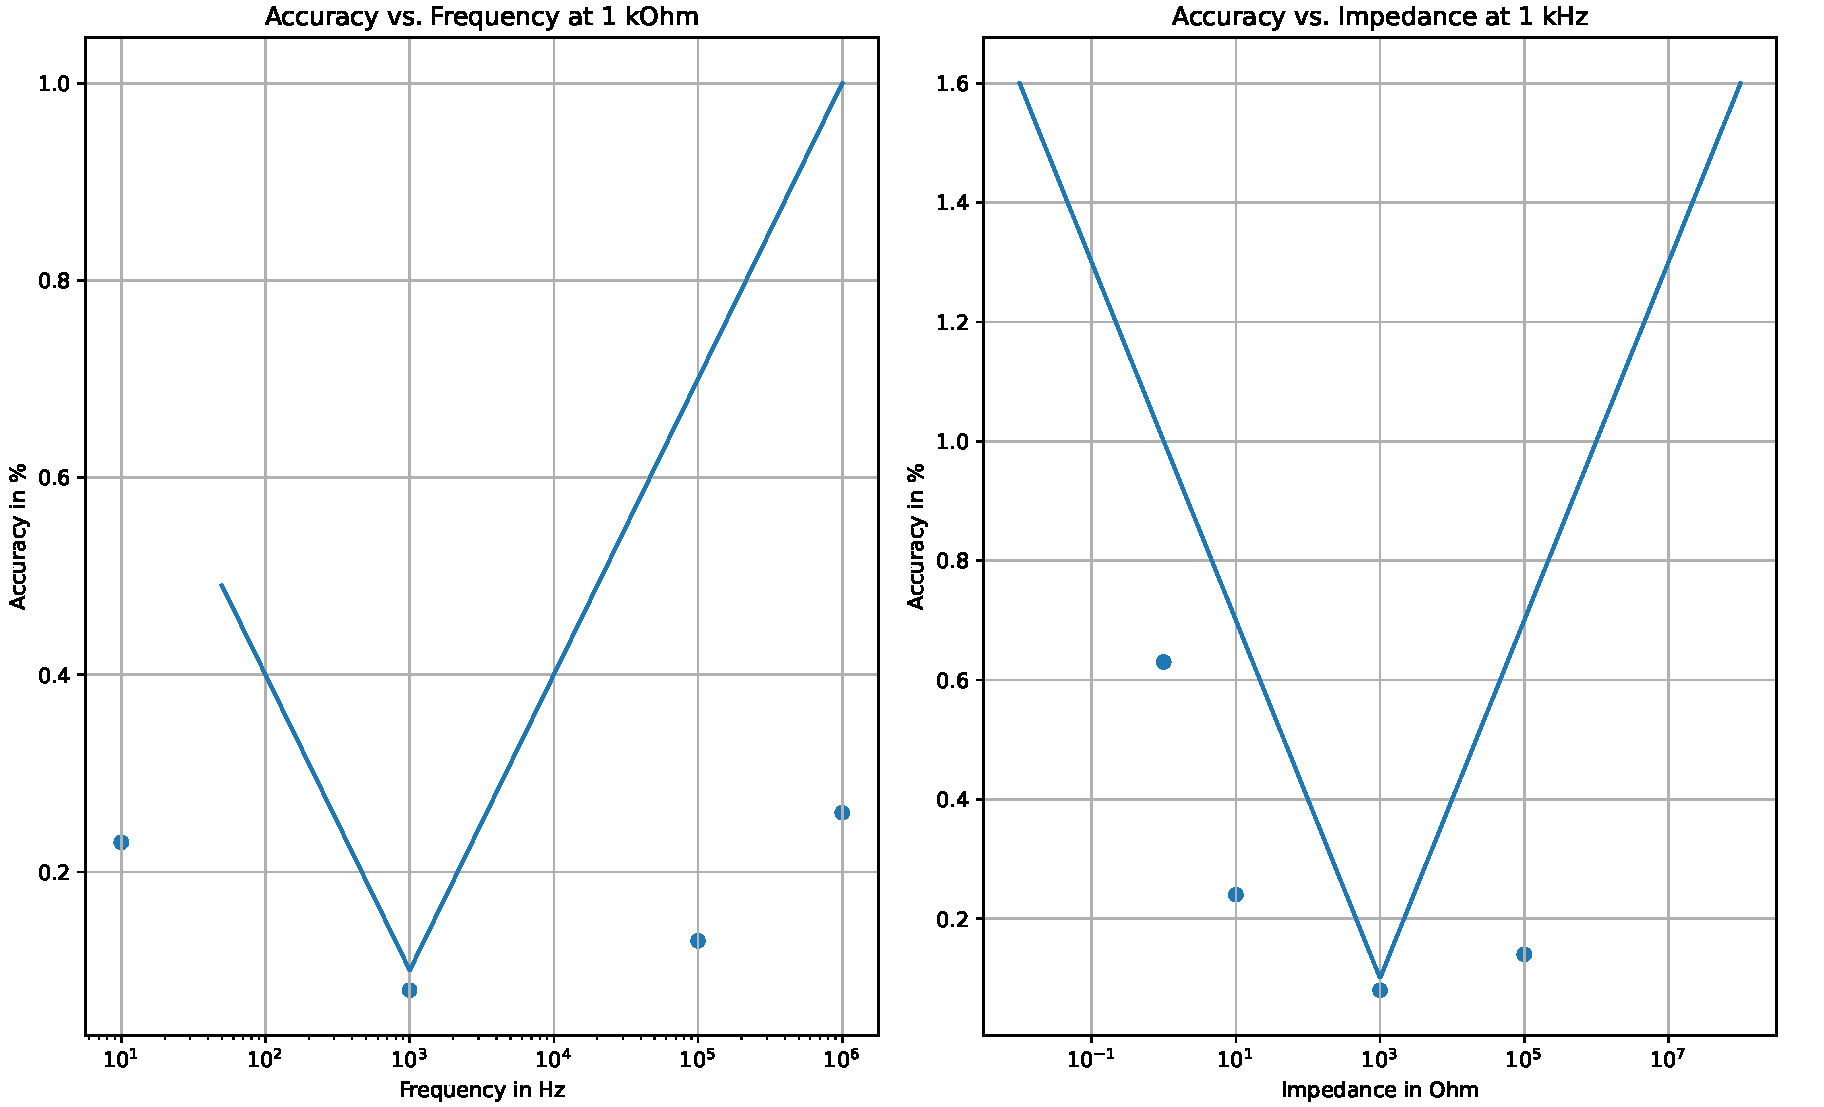
\includegraphics[width=1\textwidth]{Sections/5_SystemRequirements/Figures/ImpedanceSpec.pdf}
  \caption{Plots of the requirement for modulus accuracy, left for fixed impedance, but varying frequency, right with fixed frequency but varying impedance.}
  \label{fig_5_ModulusAccuracy}
\end{figure}

The phase accuracy is given in much the same way as for impedance. The accuracy of the phase will be dependant on the accuracy of the magnitude of the measured impedance, and as such, the phase accuracy in degrees is a function that is dependant on the impedance magnitude accuracy as can be seen in equation \ref{eq:5:A_Phi}.

\begin{equation}
  \begin{split}
    \label{eq:5:A_Phi}
    A_\phi(f_m, Z_m) & \leq \frac{180}{\pi} \cdot \frac{A_Z(f_m,Z_m)}{100} \qquad in \:degrees\\
    f_m & = Measurement \; frequency \; in \; kHz. \\
    Z_m &= Measured \; impedance \; magnitude \; in \; k\Omega.
  \end{split}
\end{equation}

Following on the previous example with an impedance of \SIQ{10}{\ohm} at a frequency of \SIQ{100}{\kilo\hertz} the impedance magnitude accuracy requirement is \SIQ{1.3}{\%} the phase
angle accuracy would be $A_(100,0.01) \leq (180/\pi)\cdot(1.3/100) = \SIQ{0.745}{\degree}$. This two variable function can also be shown as a side by side plot as seen in figure \ref{fig_5_PhaseAccuracy}.

\begin{figure}[H]
  \centering
  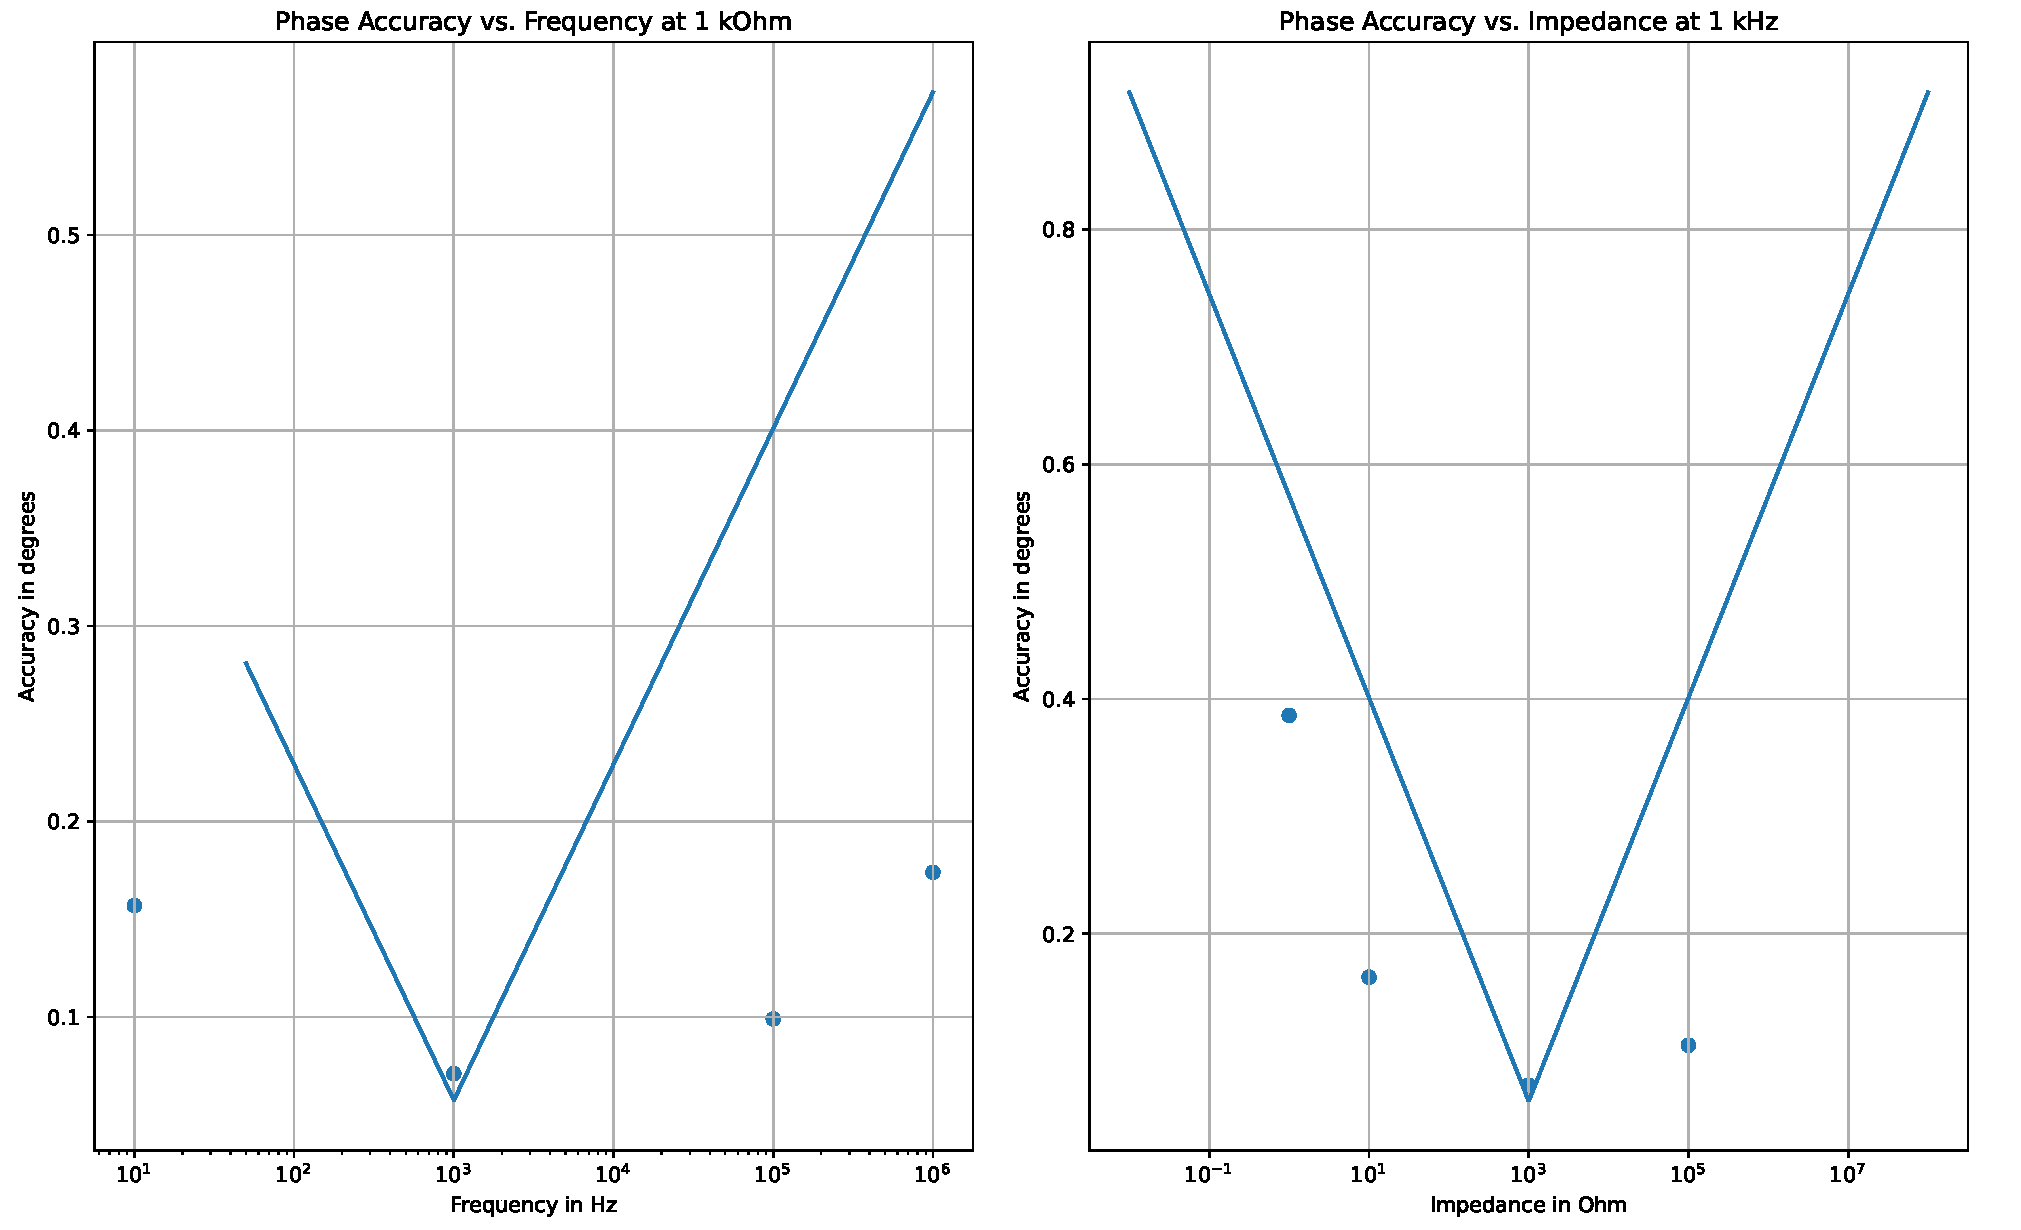
\includegraphics[width=1\textwidth]{Sections/5_SystemRequirements/Figures/PhaseSpec.pdf}
  \caption{Plots of the requirement for argument accuracy, left for fixed impedance, but varying frequency, right with fixed frequency but varying impedance.}
  \label{fig_5_PhaseAccuracy}
\end{figure}